\documentclass[aps,twocolumn,secnumarabic,balancelastpage,amsmath,amssymb,nofootinbib,floatfix]{revtex4-1}

\usepackage{graphicx}      % tools for importing graphics
\usepackage{svg}

%\usepackage{lgrind}        % convert program code listings to a form 
                            % includable in a LaTeX document
%\usepackage{xcolor}        % produces boxes or entire pages with 
                            % colored backgrounds
%\usepackage{longtable}     % helps with long table options
%\usepackage{epsf}          % old package handles encapsulated postscript issues
\usepackage{bm}            % special bold-math package. usge: \bm{mathsymbol}
%\usepackage{asymptote}     % For typesetting of mathematical illustrations
%\usepackage{thumbpdf}
\usepackage[colorlinks=true]{hyperref}  % this package should be added after 
                                        % all others.
                                        % usage: \url{http://web.mit.edu/8.13}
\setsvg{inkscape = inkscape -z -D} % conversion options for svg package, export drawing instead of page


\begin{document}
\title{Measuring dipole moment with a quadrupole magnetic field gradient}
\author{William Morse, Merritt Waldron}
%\email{nobody@mit.edu}
%\homepage{http://web.mit.edu/8.13/} %If you don't have one, just comment out this line.
\date{\today}
\affiliation{University of Southern Maine Physics Department}

\begin{abstract} 
In this experiment we set out to give the TeachSpin magnetic force apparatus its inaugural run. First we calibrated a hall effect probe and measured the on axis field of a Helmholtz coil pair in both Helmholtz and quadrupole configurations. We used these results to verify theory for the magnetic field gradient of one coil and for the constant gradient in the center of two coils in the quadrupole configuration. Next, with a calibrated spring we measure the force on a small neodymium magnet in the quadrupole field. Combining this measurement with the gradent model, we were able to find the dipole moment of the magnet. 
\end{abstract}


% edit history section!
\maketitle
% By manipulating the direction of current within each coil we can change the shape of the magnetic field inside the Helmholtz configuration. We begin by for computing the on axis magnetic field B inside our Helmholtz configuration,

\begin{figure}[here]
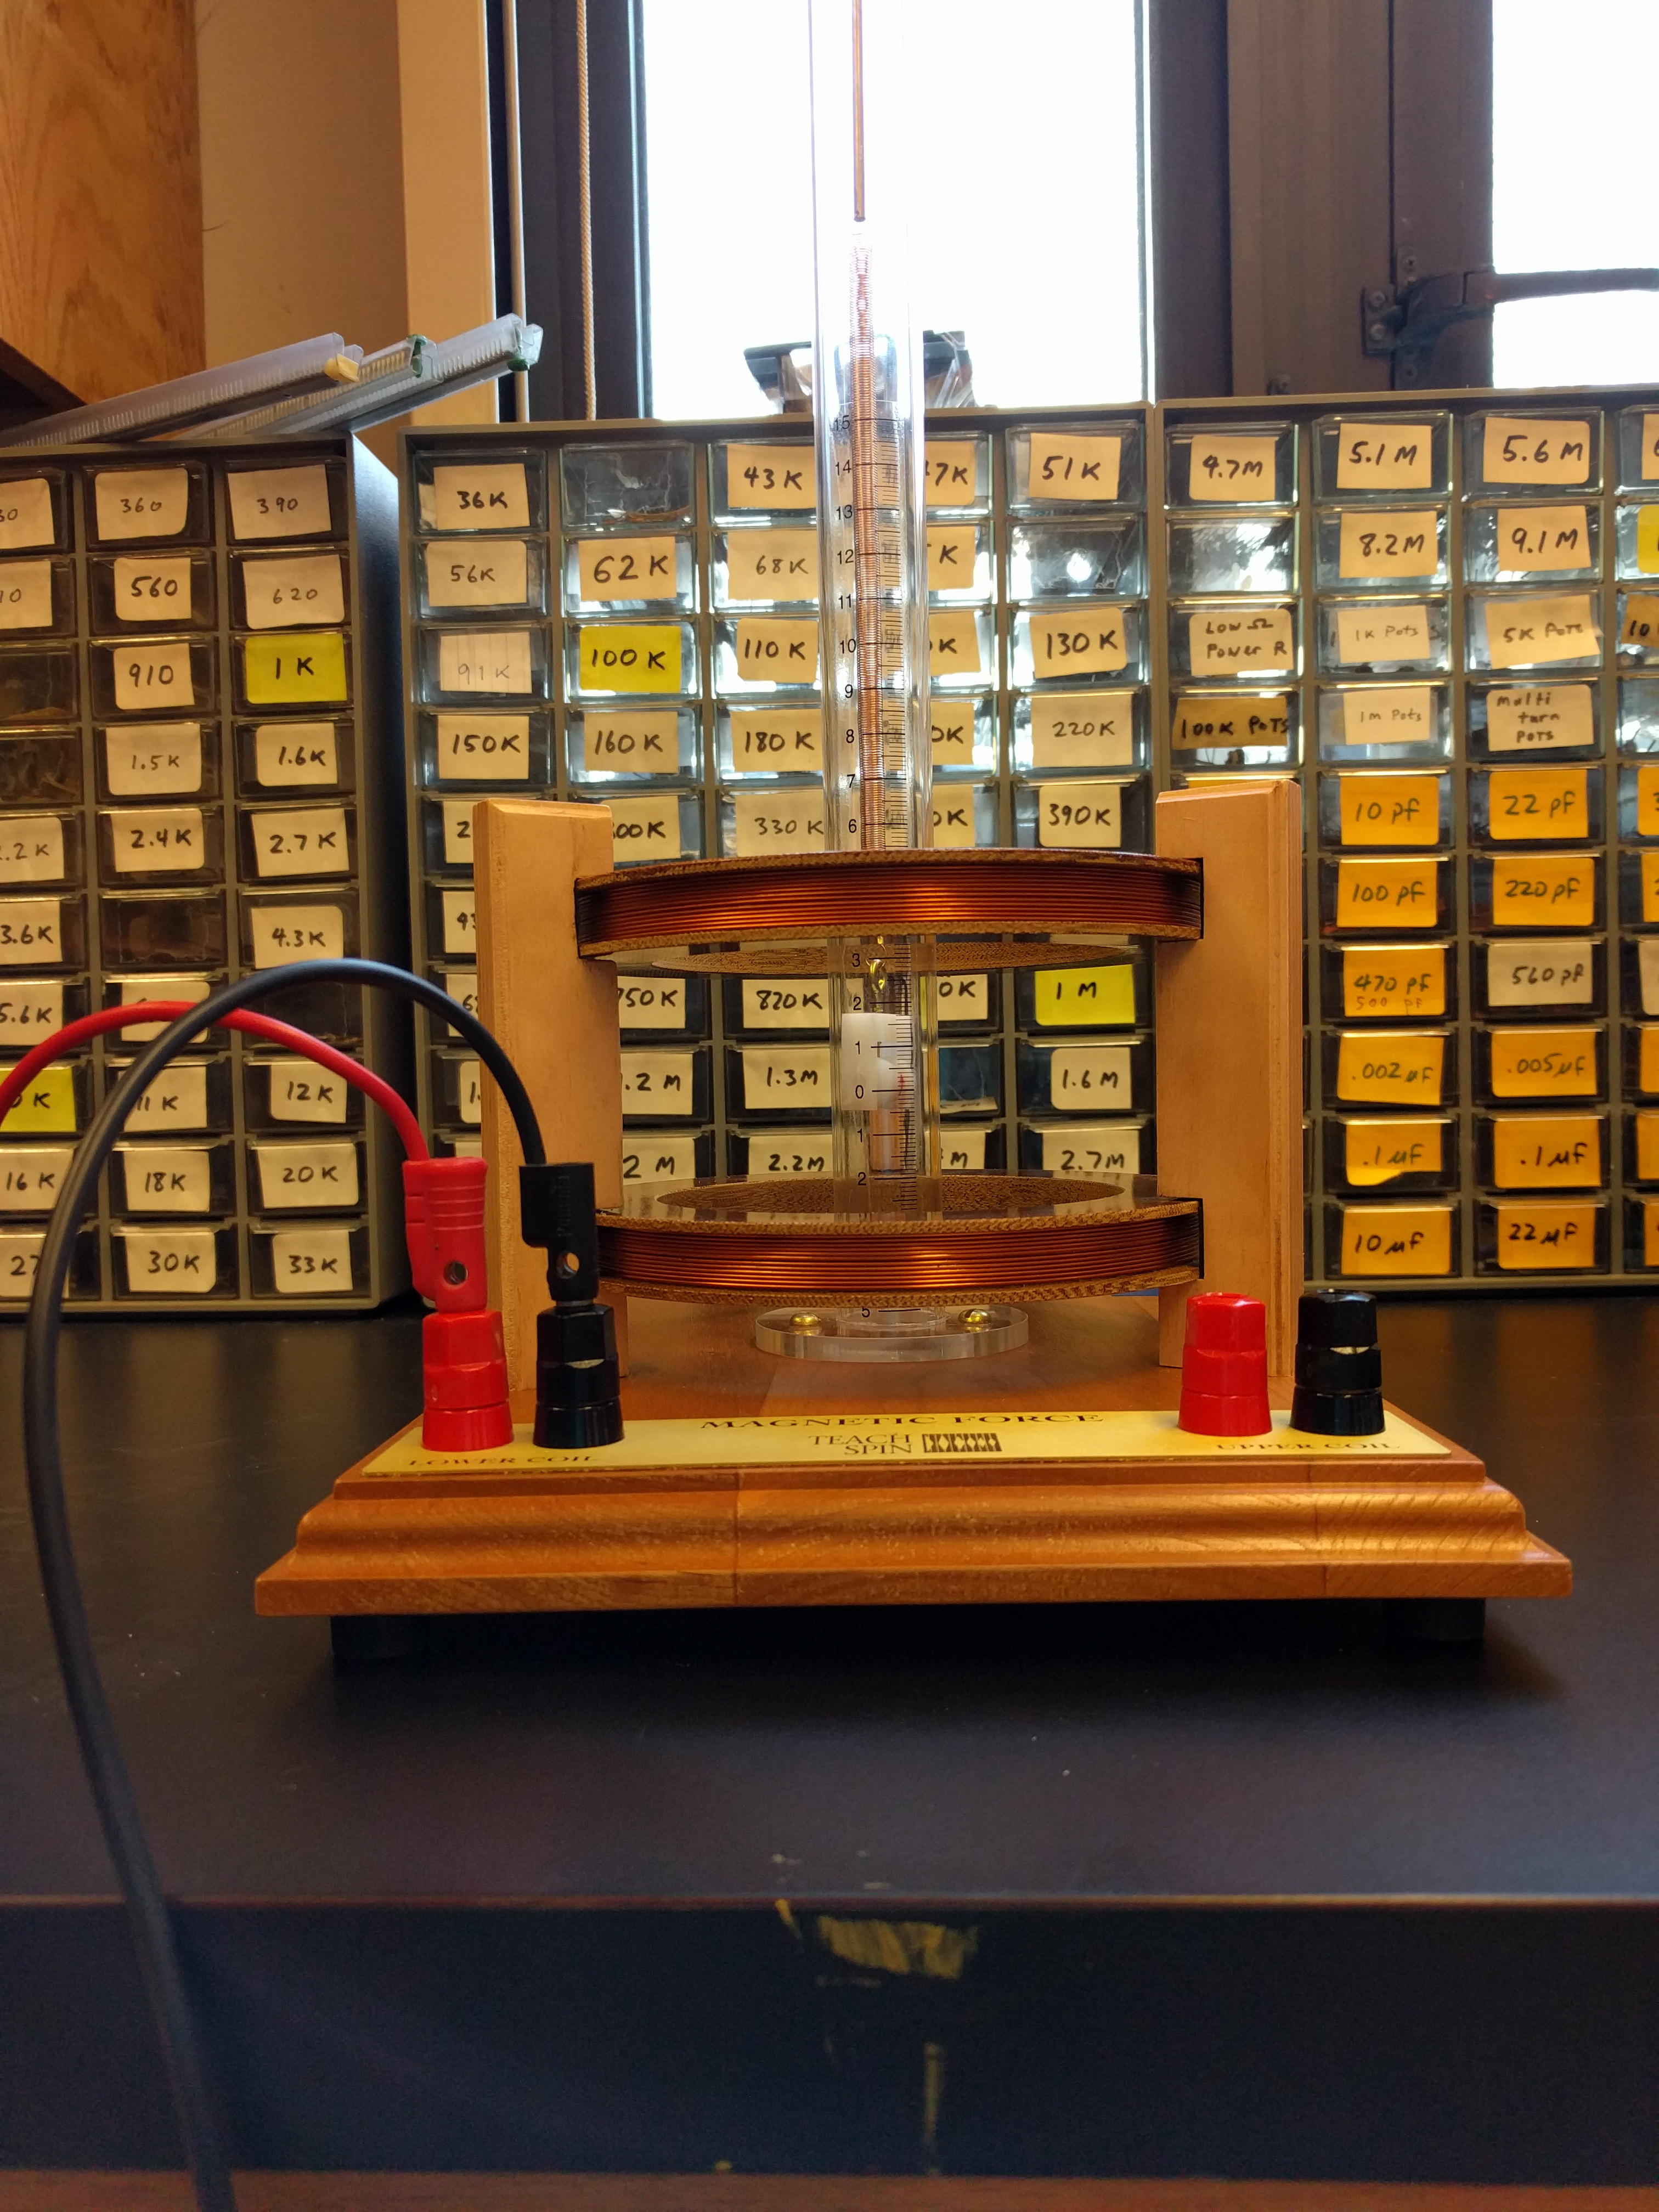
\includegraphics[width=.47\textwidth]{apparatus}
\caption{Helmholtz coils are named in honor of the German scientist Herman von Helmholtz, who, among others researched electromagnetism. Helmholtz coils are made from two identical coils with radius R. The centers of both coils are placed on the same axis distance R away from one another. In this apparatus the coils are spaced slightly more than one radius apart to compensate for the physical size of the wire and maintain a uniform field in the center.}
\label{apparatus}
\end{figure}

%There are several ways to measure magnetic fields. since the invention of SQIDs (superconducting quantum interference devices) \ref art of electronics drinking glass page there are no methods more sensitive. however squids have a high entry cost and to maintain a liquid nitrogen setup to cool the apparatus is somewhat complicated. Hall-effect sensors can measure fields with 10\% accuracy and are extremely cheap. we wanted to explore the sensitivity, noise performance, linearity and gain of a TeachSpin analog output hall sensor. the sensor claimed a gain of 1 volt per Milli-Tesla. 

\section{Hall Probe Calibration}

To calibrate our probe we wound a 575 turn solenoid. Our calibration rides on the error in the current supplied to the solenoid, the length of the solenoid as well as the field model of the solenoid: 
$$\vec B = \frac{\mu_0 N I}{L}$$ 
With the probe inserted roughly two fifths of the way into the solenoid, we took several measurements with a constant current supply. Plotting the theoretical field as a function of the sensor's output voltage gives us the gain of the sensor from a fit line. The output is linear in the range we intend to utilize in our next experiments with an rsq of $0.9999973$.  and we were able to measure the uncertainty in the calibration as: this combined with the uncertainty in our voltmeter will let us measure magnetic fields at: $\pm 0.5 \mu T$.




\section{Mapping the Helmholtz Field}
With our calibrated hall probe we measured the b field at different points along the symmetry  axis of the TeachSpin Helmholtz coil pair. We modeled the theoretical field by deriving the on axis field of one current loop and then taking a sum of the field for each wire in the apparatus.  Derived from the Biot-Savart law, the field for one loop of wire is:
$$\vec{B}=\frac{\mu_0}{2}\frac{I R_z^2}{\sqrt{R_y^2 + R_z^2}^3}$$
Where $R_z$ the radius of the loop and $R_y$ is the distance along the axis of symmetry away from the plane of the loop. \cite{knight}


\begin{figure*}[here]
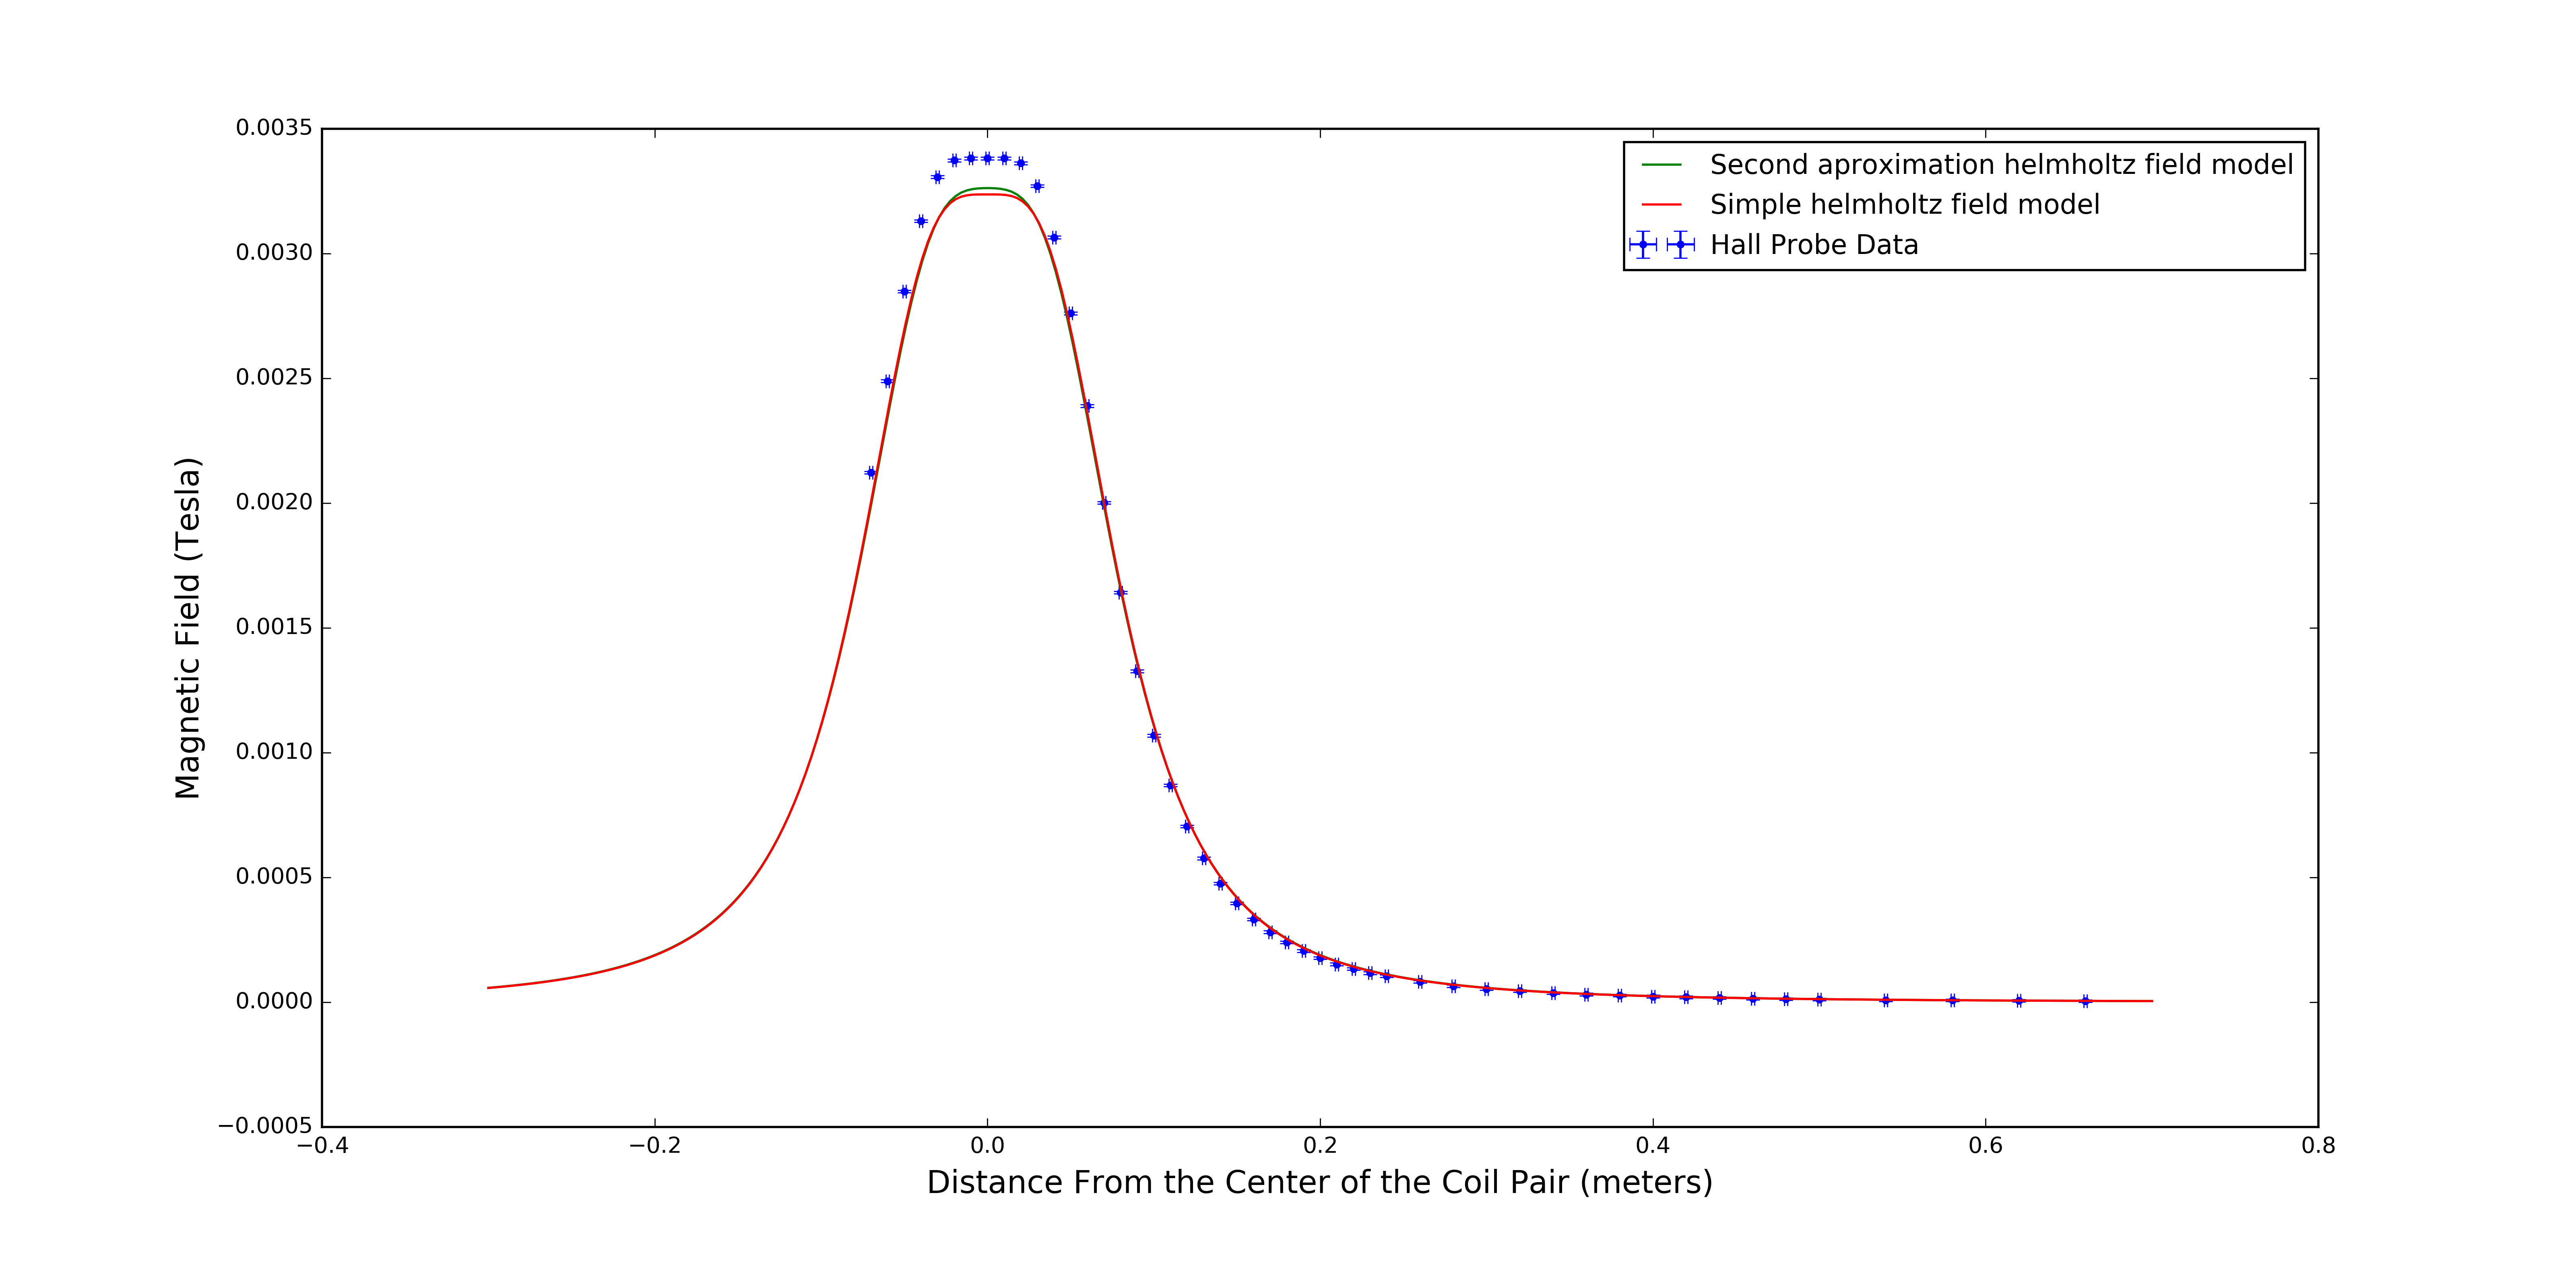
\includegraphics[width=.97\textwidth]{../DataValidation/helmholtzPlot.png}
\caption{Helmholtz configuration. The first field model used only two current loops (one for each coil). The second model splits the current over each loop of wire in the apparatus which respects the volume of each winding. The correction in the second model does little to encompass the error bars in our data.}
\label{helmPlot}
\end{figure*}


\begin{figure*}[here]
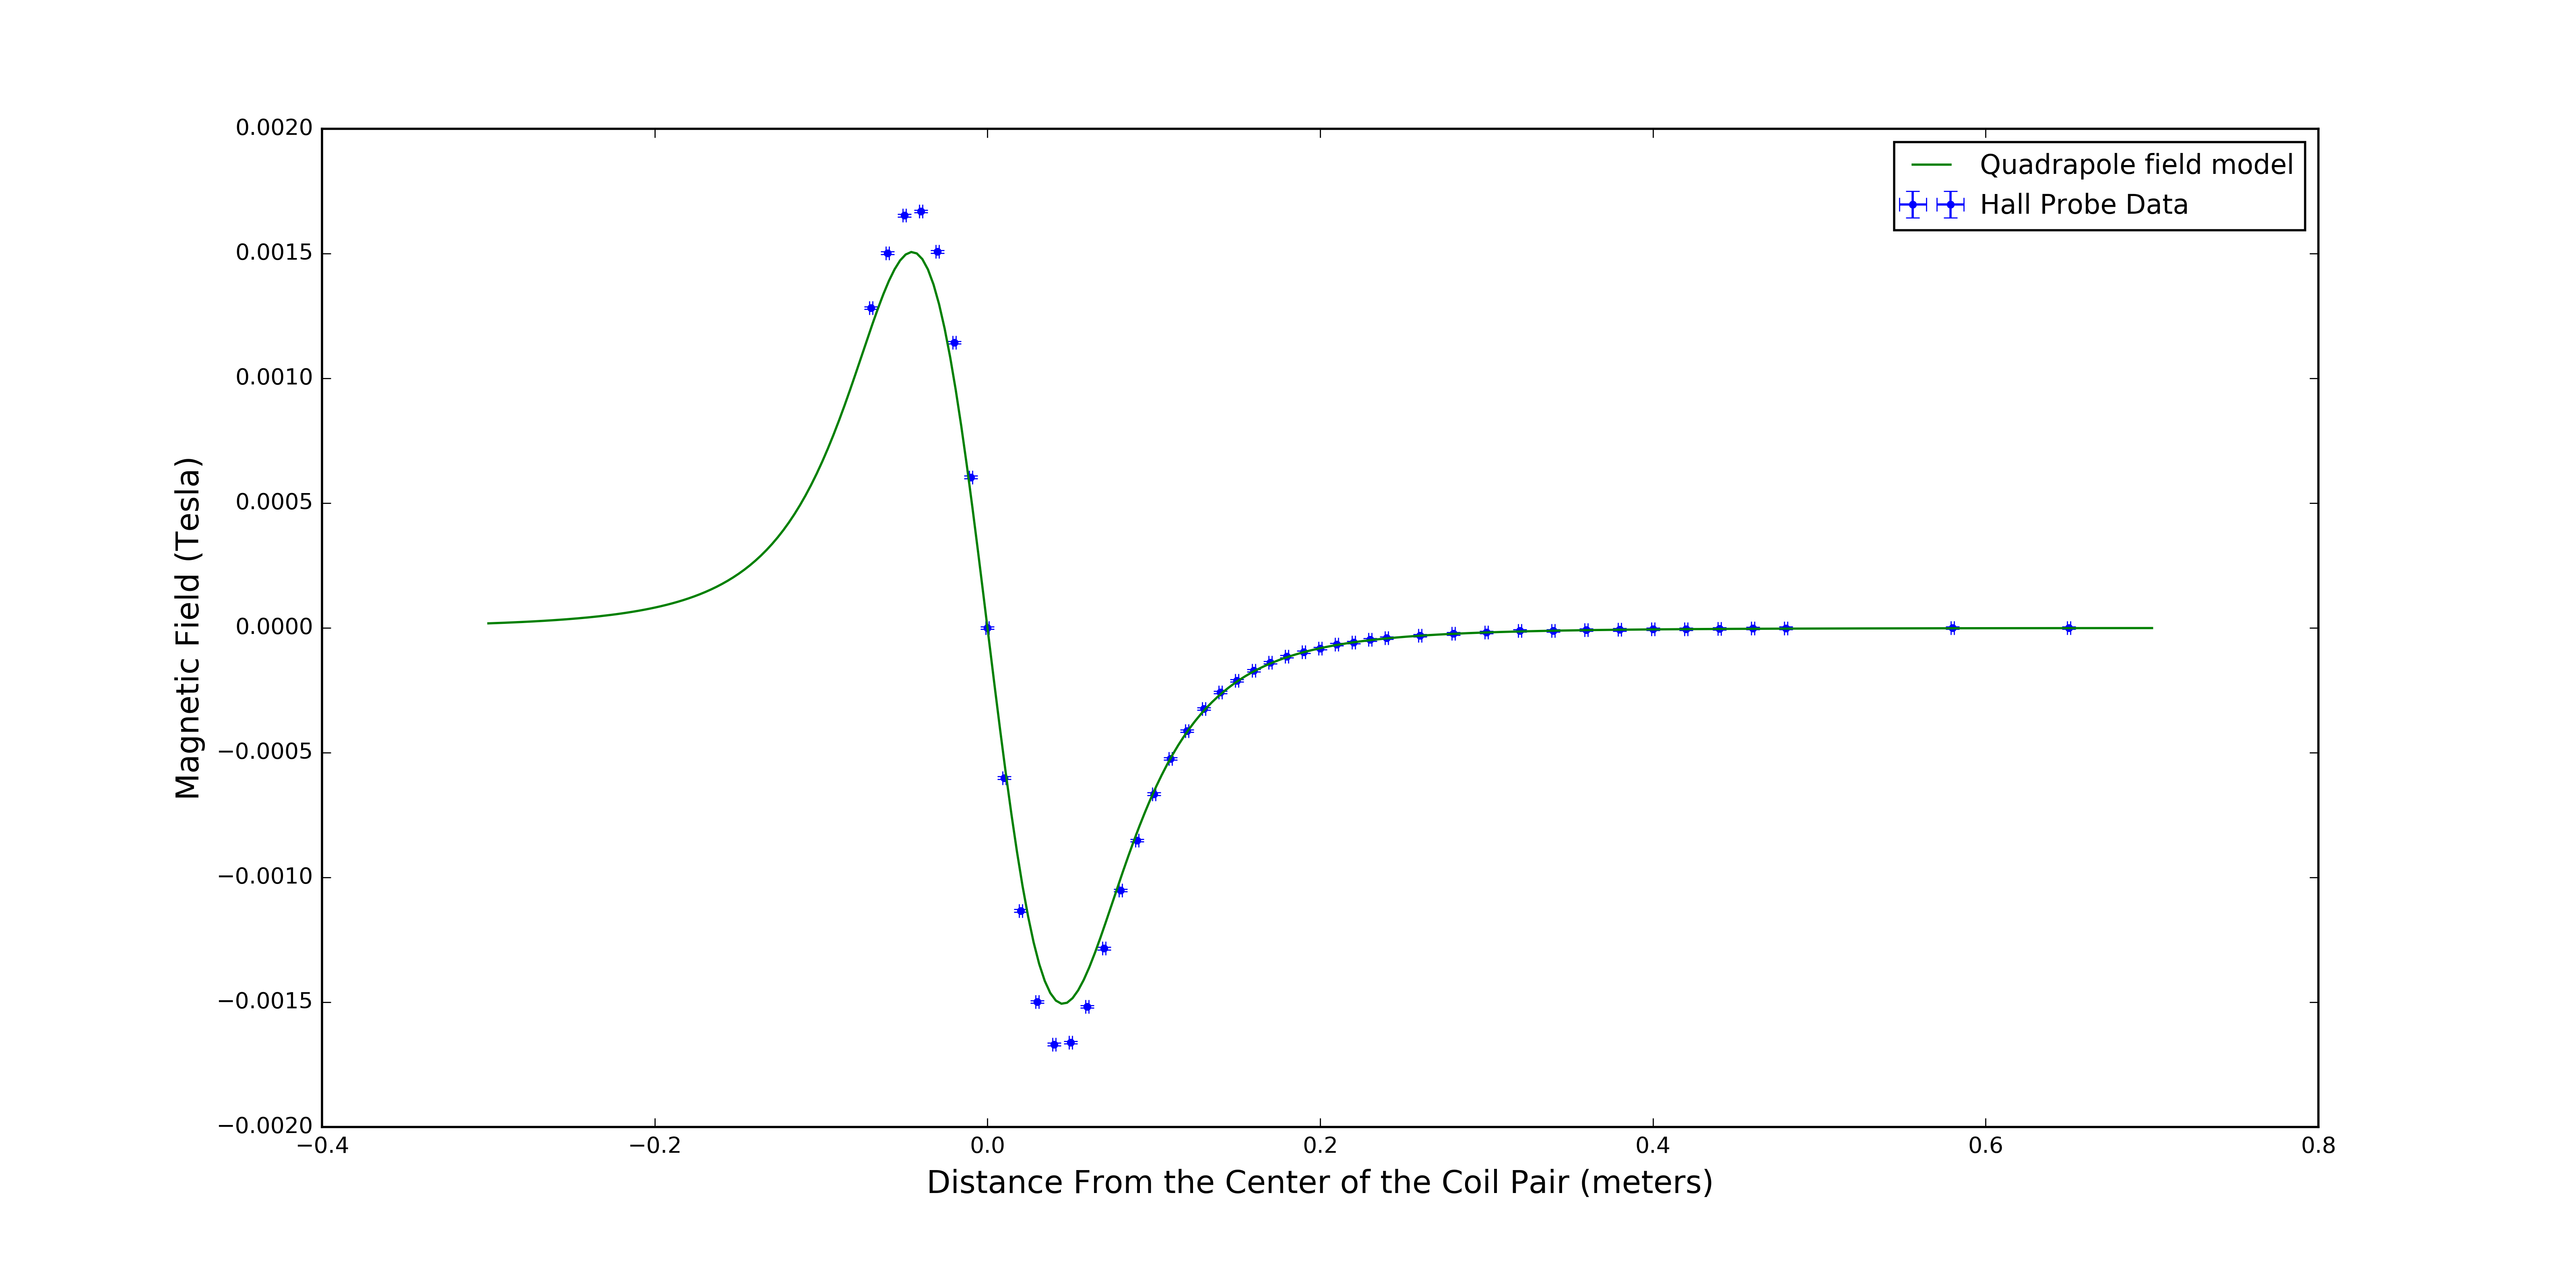
\includegraphics[width=.97\textwidth]{../DataValidation/quadPlot.png}
\caption{In quadrupole configuration the peaks also fall outside our experimental error bars consistent with what we see in the Helmholtz model.}
\label{quadPlot}
\end{figure*}

We also used the Helmholtz coils in quadrupole configuration. The only difference in the field model is that we reverse the field influence of the second coil. With the quadrupole configuration, we can get a very uniform gradient field in the center of the coil pair, which allows us to verify that the force on a magnetic dipole is proportional to the gradient in the field. 


%Additionally, this gradent gets weaker on boundaries of the uniform poriton. If the frorce on a dipole is proportional to the gradent in the field, the center of the quadrupole field will be a stable equilibrium point. 



\section{Force on a magnetic dipole}
Theory states that the force on a magnetic dipole will be proportional to the magnetic field gradient:
$$F_{dipole} = \mu \frac{d\vec B}{d R_y}$$
If we take the gradient of the magnetic field for one coil we get:
$$\frac{d\vec B}{d R_y} = \frac{-3}{2} \mu_0 N I \frac{R_z^2R_y}{(R_y^2 + R_z^2)^{\frac{5}{2}}}$$
In the center of the quadrupole field, the gradient is twice the value of the gradient due to one coil. Also with $R_y = \frac{1}{2} R_z$ the gradient at the center becomes:
$$\frac{d\vec B}{d R_{yCenter}} = \frac{-48 \mu_0 N I}{25 \sqrt{5} R_z^2}$$

We can use a spring to measure the force on a small magnet in a gradient field via Hooke's Law: 
$$F = -kx$$
Where $F$ is the restoring force of the spring, $k$ is the spring constant and $x$ is the displacement from the spring's equilibrium position. 
  To calibrate the spring we hung it inside the measurement tube. attached to the spring we hung a small magnet on a gimble. With 1 gram ball bearings we added mass to the magnet end and measured the spring's deflection. The spring had a spring constant of $1.16 \pm .07 N m^{-1}$.
  
With current flowing through the coils in quadrupole mode, we set the spring so that the magnet was centered in the uniform gradient portion of the magnetic field. The field very clearly tugged on the magnet and after turning off the power supply we measured the deflection of the spring. With the deflection we can get the force required to displace the spring from it's equilibrium position.

\begin{figure}[here]
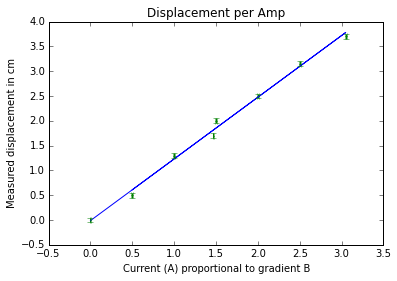
\includegraphics[width=.47\textwidth]{displacementPerAmp.png}
%\caption{}
\label{quadGrad}
\end{figure}
The displacement is proportional to the current through the coils which means the force on the dipole is proportional to the gradient field! we can solve the magnetic force equation for the dipole moment $\mu$. We found the dipole moment to be $0.391 \pm 0.005 A m^{-2}$

\section{Conclusions}
This was an excellent experiment to build intuition for magnetic fields. Dipoles,  gradients, uniform regions and stability points are ubiquitous and important concepts to understand with theory as well as in practice. The hall probe was a great tool to measure fields that are more complex to calculate in the future we would like to more fully map the off-axis Helmholtz field and perhaps attach an analog voltmeter to the sensor's output for a clearer visualization of the changes in field. The spring was sometimes prone to sticking on the side of it's containing tube, and the scale on the tube had a minimum resolution in the millimeter range which limited the resolution of our displacement measurements. With this groundwork we are ready to explore more complex field geometries and design stable magnetic interactions.

\begin{turnpage}
\begin{figure*}[here]
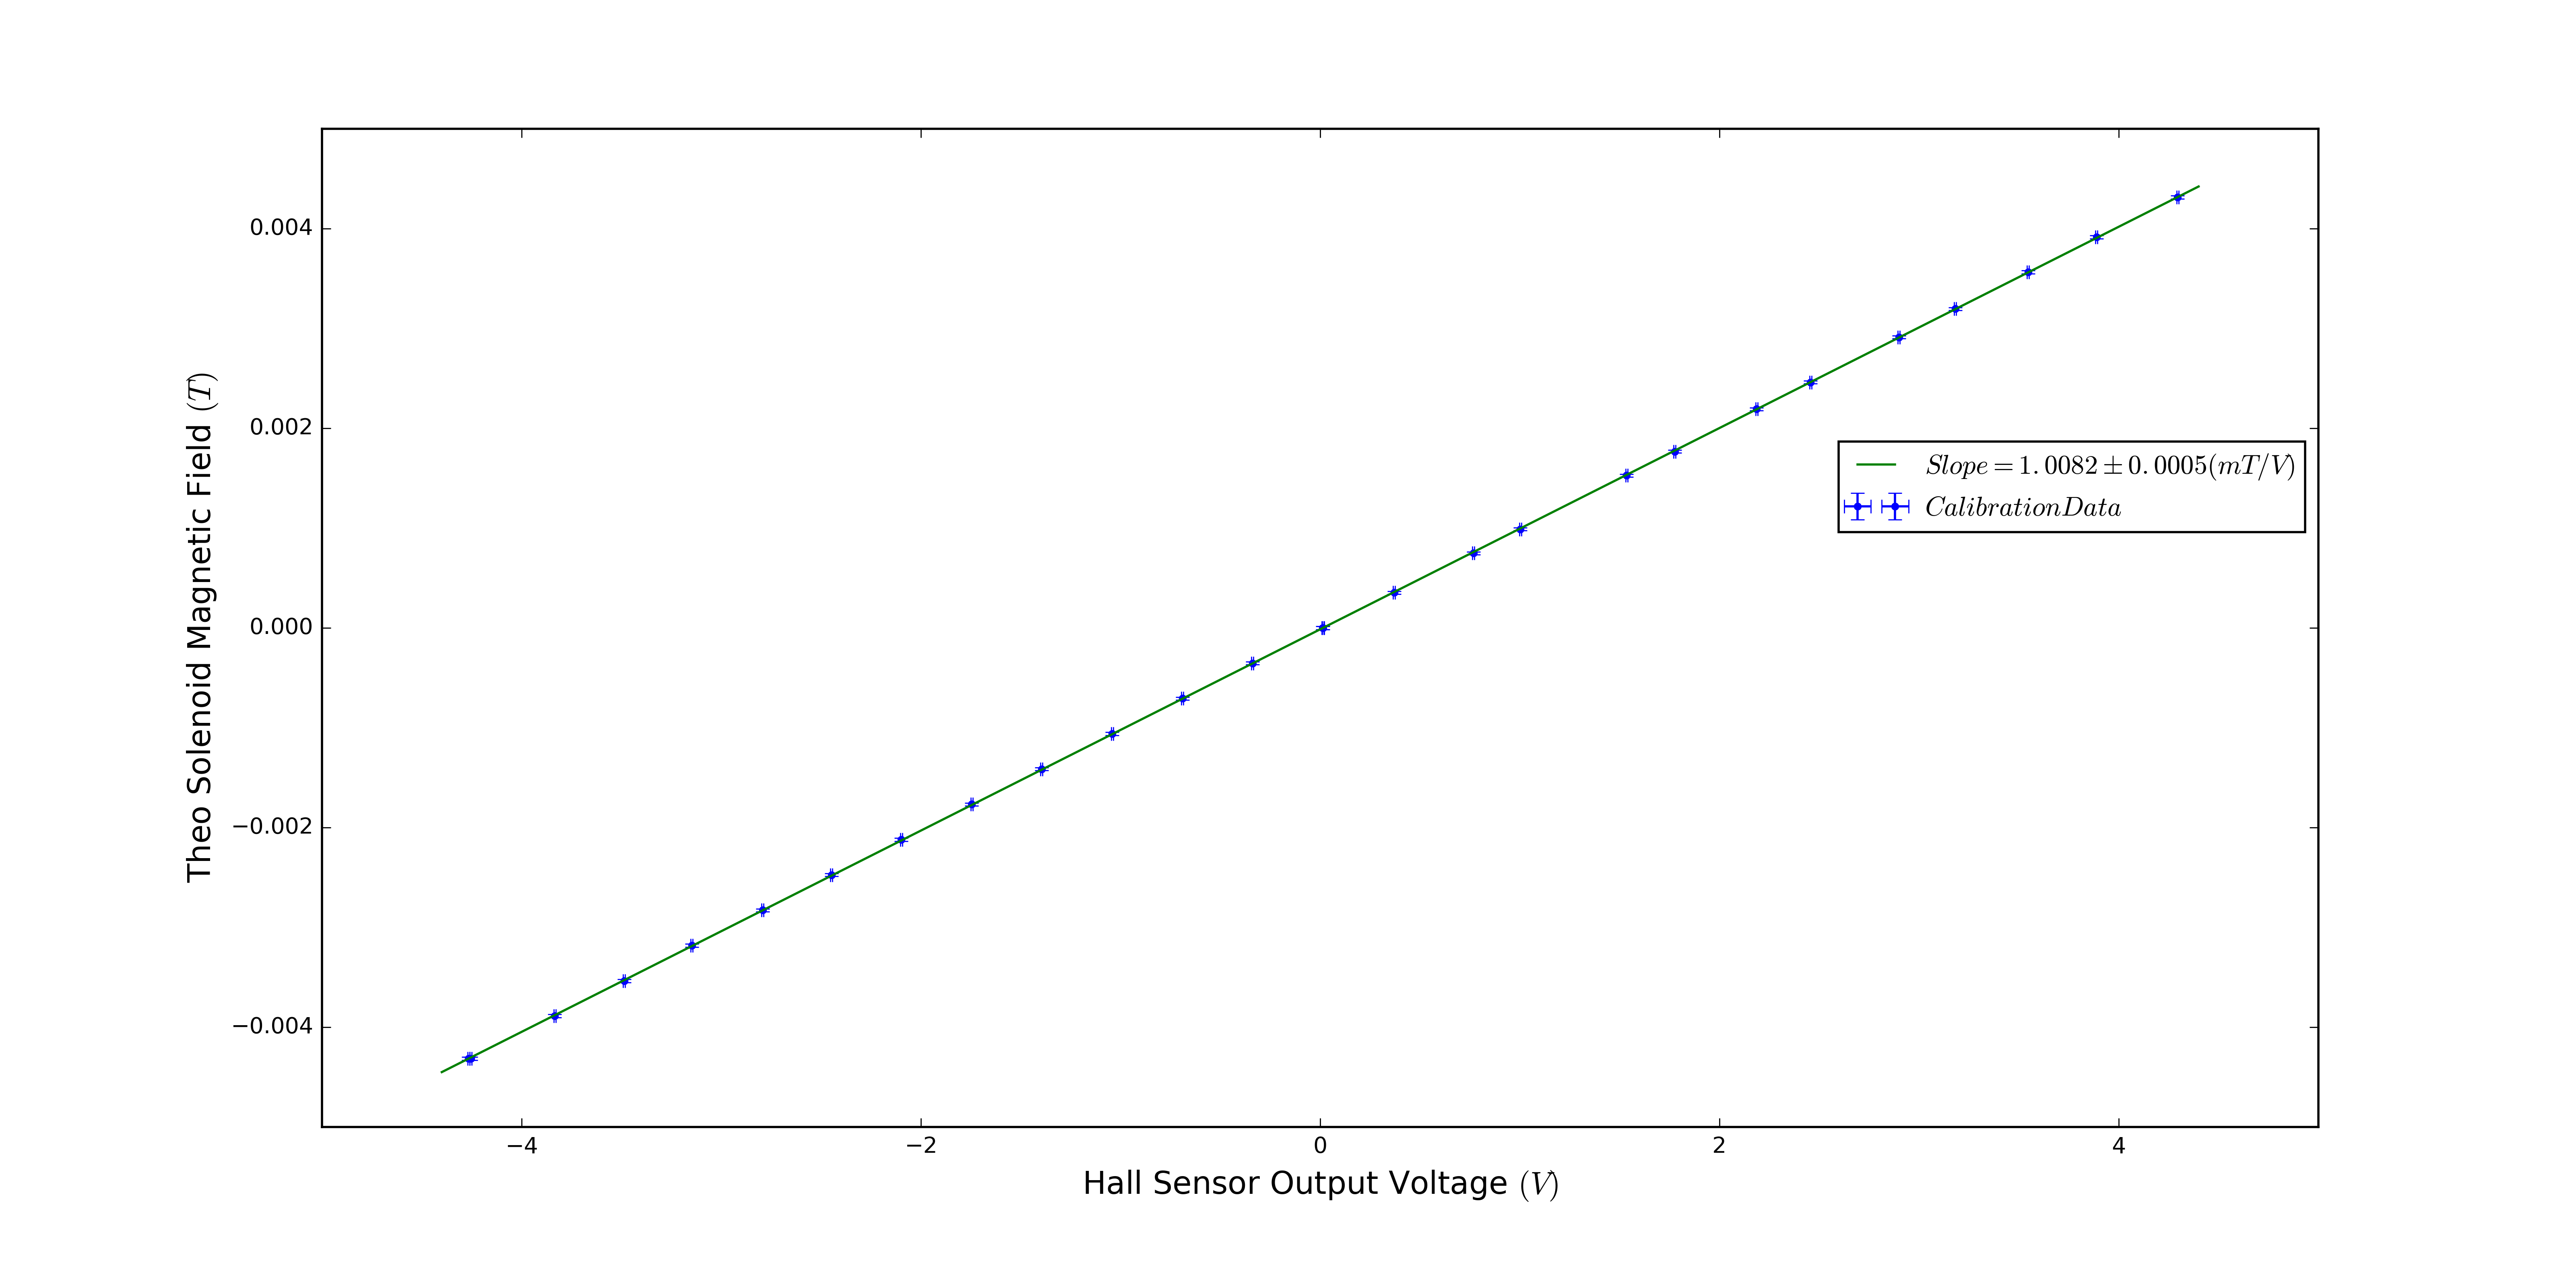
\includegraphics[height=0.77\textwidth]{../DataValidation/calibrationPlot}
\caption{Our Hall Probe calibration}
\label{apparatus}
\end{figure*}
\end{turnpage}

\begin{thebibliography}{9}

	
\bibitem{knight}
	Randall D. Knight
	\emph{Physics for Scientists and Engineers 3rd Edition}
	Pearson 2013
	
\bibitem{Higbie78}
	J. Higbie
	\emph{Off-axis Helmholtz field}
	American Journal of Physics 46, 1075 (1978)

	
	
\end{thebibliography}

\end{document}
